\chapter{Other contributions}

\section{Acoustic Novelty Detection with Adversarial Autoencoders}
\begin{figure}[h]
	\begin{subfigure}[t]{0.9\columnwidth}
		\def\svgwidth{0.5\columnwidth}
		% This file was created by matlab2tikz.
%
%The latest updates can be retrieved from
%  http://www.mathworks.com/matlabcentral/fileexchange/22022-matlab2tikz-matlab2tikz
%where you can also make suggestions and rate matlab2tikz.
%


\begin{tikzpicture}

\begin{axis}[%
width=0.85\columnwidth,
height=4cm,
at={(1.424in,0.703in)},
scale only axis,
point meta min=-156.535576728001,
point meta max=-22.4028070325664,
axis on top,
xmin=0.008,
xmax=29.992,
ytick={0,1,...,8},
x label style={at={(axis description cs:0.50,-0.06)},anchor=north},
y label style={at={(axis description cs:0.0,0.4)},anchor=south},
xlabel style={font=\color{white!15!black}},
xlabel={Time (s)},
ymin=-0.015625,
ymax=8.015625,
ylabel style={font=\color{white!15!black}},
ylabel={Frequency (kHz)},
axis background/.style={fill=white},
colormap/jet
%colorbar,
%colorbar style={ylabel style={font=\color{white!15!black}}, ylabel={Power/frequency (dB/Hz)}}
]
\addplot [forget plot] graphics [xmin=0.008, xmax=29.992, ymin=-0.015625, ymax=8.015625] {img/spectrogram-1_highlight.png};
%\draw[black,line width=2pt] (axis cs:4.7,4) ellipse (12 and 400);

%\draw[line width=1.2pt](axis cs:3.65,8) rectangle (axis cs:5.7,0);

%\node [draw, ellipse, thick, red, minimum width=14, minimum height=200, label=above:Novelty] at (axis cs:4.7,4) {};
\node[text=white] at (axis cs:4.7,4)[rotate=90] {\contour{white}{Novelty}};

%\draw[black,line width=2pt] (axis cs:18.5,4) ellipse (12 and 400);
%\draw[line width=1.2pt](axis cs:17.5,8) rectangle (axis cs:19.55,0);
\node[text=white] at (axis cs:11.6,4)[rotate=90] {\contour{white}{Novelty}};

%\draw[black,line width=2pt] (axis cs:25,0.5) ellipse (50 and 40);
%\draw[line width=1.2pt](axis cs:20,5) rectangle (axis cs:29.95,0);

%\fill[black, opacity=0.4](axis cs:20,5) rectangle (axis cs:29.95,0);
%\fill[white, opacity=0.5](axis cs:22,3) rectangle (axis cs:28.00,1);

\node[text=white] at (axis cs:25,4) {\contour{white}{Normal}};



\end{axis}
\end{tikzpicture}%
	\end{subfigure}	
	\caption{Spectrogram of an audio signal with novel and normal data.}
\end{figure}
Novelty detection is the task of recognising events the differ from a model of normality. This paper proposes an acoustic novelty detector based on neural networks trained with an adversarial training strategy. The proposed approach is composed of a feature extraction stage that calculates Log-Mel spectral features from the input signal. Then, an autoencoder network, trained on a corpus of ``normal'' acoustic signals, is employed to detect whether a segment contains an abnormal event or not. A novelty is detected if the Euclidean distance between the input and the output of the autoencoder exceeds a certain threshold. The innovative contribution of the proposed approach resides in the training procedure of the autoencoder network: instead of using the conventional training procedure that minimises only the Minimum Mean Squared Error loss function, here we adopt an adversarial strategy, where a discriminator network is trained to distinguish between the output of the autoencoder and data sampled from the training corpus. The autoencoder, then, is trained also by using the binary cross-entropy loss calculated at the output of the discriminator network.  

The performance of the algorithm has been assessed on a corpus derived from the PASCAL CHiME dataset. The results showed that the proposed approach provides an F1-score equal to 93.28\%, with a relative performance improvement equal to 0.26\% compared to the standard autoencoder. The significance of the improvement has been evaluated with a one-tailed z-test and resulted significant with $p<0.001$. The presented approach thus showed promising results on this task and it could be extended as a general training strategy for autoencoders if confirmed by additional experiments.

\subsection{Details}
In this work, we are not interested in the generative capabilities of the network, since in the novelty detection task the objective is to minimise the error made by the autoencoder in reconstructing normal data. Thus, the architecture and the training strategy are different from \cite{makhzani2015adversarial}: the discriminator network is trained to discriminate between data from a training set and data reconstructed by the autoencoder (\figref{fig:our_training}). The final layer of the discriminator is a single neuron with sigmoid activation function and its output represents the probability of the data of being sampled from the training set. At the end of the training phase, the discriminator network should not be able to distinguish training set data and reconstructed data, i.e., its output should be constantly equal to 0.5.

Similarly to \cite{goodfellow2014generative}, the training process can be viewed as a min-max game between the autoencoder and the discriminator network. Let $\boldsymbol{x}$ be an input feature vector, $\tilde{\boldsymbol{x}} = A(\boldsymbol{x})$ the output of the autoencoder, and $D(\boldsymbol{x})$ the output of the discriminator network, i.e., the probability of $\boldsymbol{x}$ of being sampled from the training data. The training procedure is composed of three main phases: the first phase and the third phase consist in updating the autoencoder and the discriminator respectively by minimising the reconstruction error and the classification error (binary cross-entropy). The middle phase incorporates the interaction between the two networks: the autoencoder weights are updated based on the output the discriminator network.


Whether a feature vector is a novel sound or a normal background sound is determined by calculating the reconstruction error, i.e., the Euclidean distance between the output produced by the autoencoder and the input data itself. If the distance exceeds a predefined threshold, the input data is classified as novelty, otherwise as normal. The threshold is calculated as follows: for each input sequence the threshold $\theta$ is calculated with the following expression:
\begin{equation}
\theta = \beta \cdot \text{median}\{e(1),\ldots,e(N)\},
\end{equation}
where $e(i)$ is reconstruction error of feature vector $i$ in the signal, $N$ is the number of features, and $\beta \in [1, 2]$ is a predefined constant.

\begin{figure}[h]
	\centering
	\begin{subfigure}[t]{0.7\columnwidth}
		\def\svgwidth{\columnwidth}
		\input{7_other_contributions/img/our_approach.pdf_tex}
		
		\caption{Proposed architecture for training an autoencoder with an adversarial discriminator network.}\label{fig:our_training}
	\end{subfigure}
	\par\bigskip
	\begin{subfigure}[t]{0.7\columnwidth}
		\def\svgwidth{\columnwidth}
		\input{7_other_contributions/img/detection.pdf_tex}
		
		\caption{Novelty detection phase.}\label{fig:our_detect}
	\end{subfigure}
	\caption{The proposed approach for novelty detection with adversarial autoencoders. For the sake of simplicity, the feature extraction stage is not shown.}\label{fig:approach}
\end{figure}

\newpage
\section[Siamese Nets for Human-Fall Detection]{Few-shot Siamese Neural Networks employing Audio features for Human-Fall Detection}

Nowadays, the detection of human fall is a problem recognized by the entire scientific community. Methods that have good performance use human falls samples in the train set, while methods that do not use it, can only work well under certain conditions. Since examples of human falls are very difficult to retrieve, there is a strong need to develop systems that can work well event with few or no data to be used for their training phase. In this work, we show a first study on few-shot learning Siamese Neural Network applied to human falls detection by using audio signals. This method has been compared with algorithms based on SVM and OCSVM, all evaluated starting from the same conditions. The proposed approach is able to learn the differences between signals belonging to different classes of events. In classification phase, using only one human fall signal as a template, it achieves about 80\% of  $ F_1 -Measure$ related to the human fall class, while the SVM based method gets around 69\%, when it is trained in the same data knowledge conditions.

\subsection{Proposed Approach}

In this work we propose a Siamese Neural Network able to learn a latent representation of an audio event. In particular, a SNN is composed of two twin networks with binded weights. A pair of inputs is provided to the system, one to each twin network. Downstream, the network maps these inputs into two different representation vectors. Then, a certain type of distance between those two representations is computed. In this work euclidean distance was used. In \figref{proposed_approach}, are reported two example of mel-spectrograms: the spectrum that is given as input to the function first network represents a chair that is overturned. The other inputs instead represent a human fall. As can be seen, the signals are not distinguishable at a glance, thus we think that the differential approach of the SNN, described below, seems to be appropriate.

Our Siamese network has been trained on a corpus of labelled object fall events and not including any human fall. Pairs of events belonging to the same class correspond to the positive examples while pairs of events belonging to the different class a negative one. In particular, the term few-shot comes from the fact that although, in this case study, human falls have not been used for training, some of them are used in the optimization phase, before the final test.
\begin{figure}
	\centering
	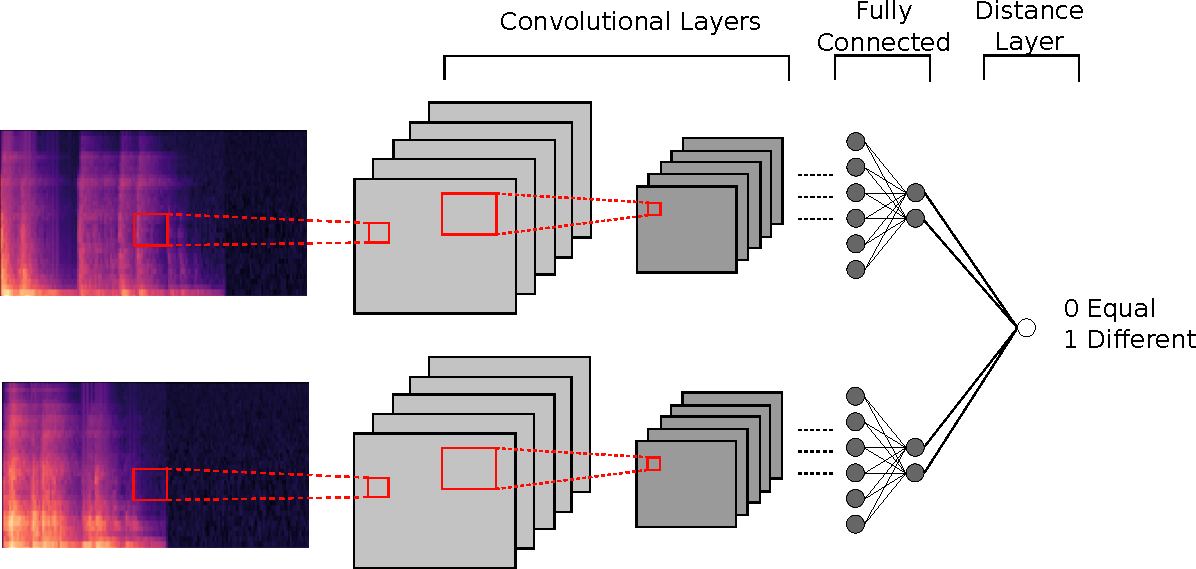
\includegraphics[width=0.7\linewidth]{img/Siamese_approach}
	\caption[Siamese Nets for human-fall detection]{Proposed approach for Human-Fall Detection.}
	\label{proposed_approach}
\end{figure}

\subsection{Results}
The results obtained for each method are reported in \figref{fig:results_f1}. The figure shows the $ F_1 -Measure$, false negative rate (miss rate) and false positive rate (false alarm rate) referred to the human fall class. It is clear that the supervised SVM method outperforms all other in terms of  $ F_1 -Measure$ as expected. The OCSVM instead is the worst method if used in this context, because its training procedure does not include any human fall, but the normality model is composed of others types of falls, making it difficult to identify the human fall as ``novelty''. The Siamese and the SVM-unbalanced, which start from the same data for the training, are classified in the intermediate positions as expected. However, we note that the proposed approach achieves a better result, exceeding the $ F_1 -Measure$ of SVM-unbalanced of about 11\%. 

\begin{figure}[h]
	\centering
	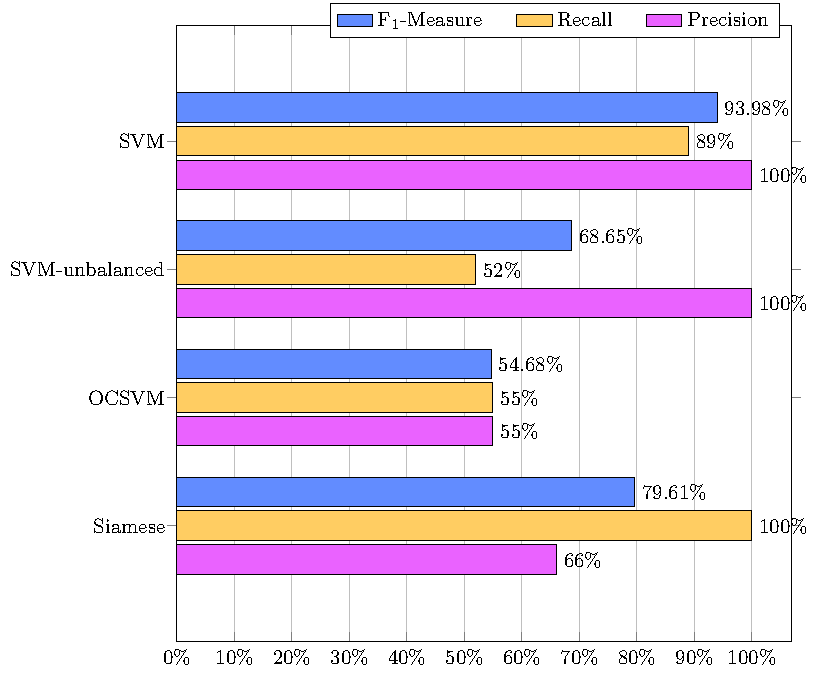
\includegraphics[width=0.7\linewidth]{img/results_f1}
	\caption[Siamese Nets for human-fall detection - Results]{$F_1 -Measure$, precision and recall: the metrics are referred to the human fall class}
	\label{fig:results_f1}
\end{figure}

\newpage
%%%%%%%%%%%%%%%%%%%%%%%%%%%%%%%%%%%%%%%%%%%%%%%%%%%%%%%%%%%%%%%%%%%%%%%%%%%%%%%%%%%%%%%%%%%%%%%%%%%%%%%%%%
\section{Generative Raw Audio Synthesis}